\chapter{Simulation study}
After developing FHTBoost (see chapter \ref{ch:FHTboost}), we wish to verify that it works, i.e. that it has predictive power and selects correct variables.
Not only that, but we wish to see which of the two versions of the algorithm works best, namely the fixed intercept version and the version with an iteratively changing intercept.

One way to verify that a statistical estimation method works, is to test it on simulated data.
Simulation studies are used for many different purposes, but a particularly common purpose is to simulate survival data from the ``true model'' (in this case, our first-hitting-time model), for which we know the true values of the parameters.
We can then use our developed method to estimate these parameters, and see how well it recovers the true parameters in the final model, and how well the model fits the simulated data.
The model should fit the simulated data well, because the data generating mechanism \textit{is} the model.
In this chapter, we simulate data, use FHTBoost to estimate models, and assess the performance of these models.
The boosting algorithm has two main purposes:
Selection of variables, and minimizing test error.
To assess the test/generalization error, we calculate the difference of deviance on the test set.
To assess variable selection, we look at some well known metrics.

\section{Simulation design}
In this chapter we describe two scenarios, a highly correlated scenario and an uncorrelated scenario. 
The purpose of each scenario is to first generate survival data from an FHT mechanism, based on known true parameters, then use FHTBoost to estimate the parameters of the model, and then finally to assess the model's performance on this data.
In both scenarios, we generate a high-dimensional covariate matrix $\X$ consisting of covariate vectors
\begin{equation}
    \x_1,\x_2,\ldots,\x_{p_1},
\end{equation}
which is supposed to mimic gene expression data.
We also have a low-dimensional covariate matrix $\Z$, which similarly consist of covariate vectors
\begin{equation}
    \z_1,\z_2,\ldots,\z_{p_2},
\end{equation}
and which is supposed to mimic clinical measurements.
The motivation for this dichotomy is discussed in subsection \ref{subsec:FHT-combine}.
We link each covariate to a parameter in a parameter vector.
We let $\X$ correspond to $\bbeta$, and $\Z$ correspond to $\bgamma$.
This allows us to test the variable selection performance of FHTBoost.
In each parameter vector, we set only a small number of parameters to a non-zero value, and we set all the rest to zero.
Thus only a very small number of covariates will have an effect.
Given these parameter vectors and covariate matrices, we calculate a specific $y_{0,i}$ and a specific $\mu_i$ for each individual $i$, where $i=1,2,\ldots,N$, and where $N$ is the size of the data set.
From the FHT perspective, discussed previously in section \ref{fht-idea} and onward, these are parameters representing the health process of each individual.
To reiterate, an individual $i$ has a stochastic health process, specifically a Wiener process with an initial level $y_{0,i}$ and a drift $\mu_i$.
When the health process hits 0, it causes the event for the individual.
Since the FHT of a Wiener with health level $y_{0,i}$ and drift $\mu$ is $\IG(y_{0,i},\mu_i)$, then also the individual's lifetime follows this distribution $\IG(y_{0,i},\mu_i)$.
This relationship allows us to easily draw a lifetime for each individual from its respective inverse Gaussian distribution.

It is important to evaluate an estimated model's performance on a separate and unseen test set.
Each training set will be generated by drawing $N=500$ individuals as described above, with a specific seed.
Since we are simulating, it is simple to generate a test set by drawing from a unique seed.
We are therefore also able to decide the size of the test set.
We set $N_{\text{test}}=1000$ observations.

We generate $B\approx500$ data sets by drawing survival data according to algorithm \ref{algo:FHT-sim}.
In each data set there are $N=500$ observations. 
We treat each data set as a separate training data set.
To estimate a model based on a training set, we first perform repeated 5-fold cross validation procedure (see subsection \ref{subsec:K-fold}), with 5 repeats.
As shown in subsection \ref{subsec:iterations}, this provides a reasonably variance reduced estimate of $\mstop$ (near the ``true'' $\mstop$).
We then estimate a model based on the entire training set, by running FHTBoost with $\mstop$ number of iterations.

To simulate the covariate matrices $X$ and $Z$ we will use Algorithm \ref{algo:clinical-sim}, which is a method for simulating clinical and gene data together.
We specify the different correlations for the covariate matrices.
We specify the true parameter vectors, $\bbeta$ and $\bgamma$.
For each scenario, we create $B$ data sets.
For each of these, we estimate FHT parameters using FHTBoost.

For each data set $D_b$, we first draw data (with a specific seed to ensure reproducibility).
We do this by drawing covariate matrices $\X$, $\Z$ from Algorithm \ref{algo:clinical-sim}.
Then we combine these with the true covariate matrices to get vectors $\y_0$ and $\mathbf{\mu}$ of initial value of the health process, and drift, respectively.
Then we draw from the Inverse Gaussian distribution according to Algorithm \ref{algo:FHT-sim}, obtaining $N$ right-censored lifetimes, i.e., $N$ tuples $(t_i,d_i)_{i=1,\ldots,N}$.
With these tuples, then, we can do a run with the FHT boosting algorithm. We first use repeated K-fold cross-validation to find the optimal number of boosting steps, $m_{\text{stop}}$.
Then we estimate the model on the whole of this training set.
Then we validate this model on a test set of size $N_{\text{test}}$.
The data here are drawn in the exact same manner as the training data, again with a specific seed for reproducibility.
We first discuss the algorithms we use to generate FHT survival data.

\section{Simulation of survival data from an IG FHT distribution}\label{sec:simulate-IG-data}
We wish to simulate survival times $(\ti)_{i=1}^N$ with censoring.
We first draw $N$ uncensored survival times $\{\tilde{t}_i\}_{i=1}^N$ from a survival time distribution $f(\cdot)$.
If this distribution has a closed form probability distribution function, we can draw from it directly, and this is the case for us.
To implement censoring of the data, we draw censoring times $w_i\sim f(\cdot),i=1,\ldots,N$ from some other lifetime distribution where the parameters do \textit{not} depend on covariates.
Thus the observed survival times are
\begin{equation}
    t_i=\min(\tilde{t}_i,w_i),
\end{equation}
as we have seen before.
The corresponding censoring indicator, $d_i$, is then set equal to 1 if the actual survival time was observed, i.e., if $\ti<w_i$.
We end up with a data set
\begin{equation}
    D=(\x_i,\,\z_i,\,t_i,\,d_i)_{i=1}^N.
\end{equation}
Note that this prcedure simulates censored time under independent censoring, since indeed the censoring times are independent of the survival times.
See \ref{algo:FHT-sim} for a schematic overview of the algorithm.

\begin{algorithm}
\caption{Generating survival data from Inverse Gaussian FHT distribution}
\label{algo:FHT-sim}
\begin{enumerate}
    \item Obtain the design matrices $\X$, $\Z$ and the true parameter vectors $\bbeta$ and $\bgamma$.
    \item\label{algo:FHT-sim-step-cens} Specify a censoring time distribution.
    \item Calculate the distribution parameters $y_0$ and $\mu$ using the link functions,
        \begin{align*}
            y_0&=\exp(\bbeta^T\X)=\exp\left(\beta_0+\sum_{j=1}^p\beta_jx_j\right), \\
            \mu&=\bgamma^T\Z=\gamma_0+\sum_{j=1}^d\gamma_jz_j.
        \end{align*}
    \item Draw $N$ uncensored survival times $(\tilde{t}_i)_{i=1}^N$ from $\IG(\boldsymbol{\mu},\boldsymbol{y}_0)$, where
        \begin{equation*}
            \tilde{t}_i\sim\IG(\mu_i,\y_{0,i}).
        \end{equation*}
    \item Draw $N$ censoring times $(w_i)_{i=1}^N$ from the censoring time distribution specified in step \ref{algo:FHT-sim-step-cens}.
    \item Right censor the survival times by choosing
            \begin{equation*}
                t_i=\min(\tilde{t}_i,w_i).
            \end{equation*}
          The censoring indicator on whether observation $i$ was observed or not is then
          \begin{equation*}
            d_i=I(t_i=\tilde{t}_i).
          \end{equation*}
    \item The simulated data set is $D=(t_i,\,d_i)_{i=1}^N$.
\end{enumerate}
\end{algorithm}

\section{Generating correlated clinical and gene expression data}
To create a realistic scenario where we have data looking like gene expression data and clinical data, we need to define a proper correlation structure.
We can draw covariate matrices from a normal distribution with a suitable covariance matrix.

We consider a scenario where we have a covariate matrix $X$ consisting of $p$ gene expressions, and a covariate matrix $Z$ consisting of $d$ clinical measurements.
We can imagine that some of the genes in $X$ are highly correlated.
One way to imagine this is to imagine that we have blocks of genes,
where inside one block, the genes are highly correlated, whereas genes in one block are not correlated to other genes.
In addition, one block of genes might affect a block of clinical variables as well.

We specify a number of blocks $B$. A given block $b,b=1,2,\ldots,B$, contains a certain number of genes, $G_b$, which are correlated to each other.
It also contains a certain number of clinical measurements, $C_b$. These measurements are correlated to each other, and to the genes in the block.

After setting up the block structure, we 
\todo[inline]{Finish this}

There are three types of correlations.
1. Within each block of genes. Defaults to 0 for genes not belonging to any block.
2. Between clinical predictors in each pathway
3. Between the clinical and molecular predictors in each pathway

Algorithm \ref{algo:clinical-sim} contains a schematic overview.

\begin{algorithm}
\caption{Generating correlated clinical and gene expression data}
\label{algo:clinical-sim}
\begin{enumerate}
    \item Lorem ipsum.
\end{enumerate}
\end{algorithm}

\section{Scenarios}
\subsection{Scenario 1: Uncorrelated case}
We generate a data set of size $N_{\text{scenario}}=500$, and parameter vectors of size $10000$ and $15$, respectively.
We let $\bbeta$ be a large vector of size $p=10001$, and $\bgamma$ be a small vector of size $d=16$.
We first discuss the size of the parameter effects.
The parameter vector $\bbeta$ is linked to the initial level $y_0$ by an exponential link function.
Consequently, each parameter effect is \textit{multiplicative} instead of additive.
A large gene expression value can therefore potentially cause a large change in $y_0$.
Since there are 35 elements of $\bbeta$ which are informative, there is a reasonable chance of such extreme values occurring in $y_0$.
Because of this, we had trouble setting up simulations in which there was much signal from the underlying parameter vector.
Therefore we choose 0.1 for the informative parameter effects $\beta_j,j=1,2,\ldots,35$.
The parameter sizes on the drift might also appear rather small, at 0.1, but this effect is linear with time.
By having a relatively low effect per time unit, we ensure that the lifetimes are not too short.
These two considerations in mind made us achieve a decent simulation setup.
Specifically, we set the intercept term in $\bbeta$ to be 2.0, and the following $p_1=35$ elements to be 0.1.
We set all other elements to 0.
For $\bgamma$, we set the intercept term to be -1.
In similar fashion as in $\bbeta$, we let the first 5 elements in $\bgamma$ have a non-zero value of -0.1, while we set the remaining 10 elements to 0.
Hence, the true parameter vectors are
\begin{align*}
    \bbeta=\left(2.0, \underbrace{0.1, 0.1, \ldots, 0.1}_{\text{length 35}}, \overbrace{0, 0, \ldots, 0}^{\text{length 9965}}\right) \\
    \bgamma=\left(-1.0, \underbrace{0.1, 0.1, \ldots, 0.1}_{\text{length 5}}, \overbrace{0, 0, \ldots, 0}^{\text{length 10}}\right)
\end{align*}
We draw $X$ and $Z$ from Algorithm \ref{algo:clinical-sim} for drawing clinical and gene data, with $B=0$ blocks.
We specify that all correlations are 0, meaning no covariate correlates with any other.
We generate $B=500$ data sets from this algorithm, where we set the seed at the beginning of each simulation.
Having now a data set $D_b$, we run cross validation on this data set to find the optimal iteration number $m_{\text{stop}}$.
We then run a boosting algorithm with $m_{\text{stop}}$ steps on the training set, to estimate parameters.
We will discuss the results in the next section, but we first describe the other scenario.

\subsection{Scenario 2: Correlated}
Consider now a scenario where we wish to have high correlation.
We have blocks of genes which are correlated, meaning the genes comprising one are correlated.
Furthermore, we let the genes in a block of genes be correlated with a (smaller) block of clinical measurements.
Finally, the clinical measurements are correlated.
All these correlations are set to 0.7.
The main purpose of the algorithm is to specify the covariance matrix before drawing the data.

There are three types of correlations.
1. Within each block of genes. Defaults to 0 for genes not belonging to any block.
2. Between clinical predictors in each pathway
3. Between the clinical and molecular predictors in each pathway

\section{Results}
After having estimated an FHT model on the training set, we assess the performance of the model on the test set.
We calculate the difference of deviance.
To assess the variable selection of the model, we calculate metrics for the variables selected based on the training set.
We count $TP$, the number of informative covariates which were selected in the estimated boosting model, and $TN$, the number of non-informative covariates which were selected in the model.
Based on these numbers, we calculate the metrics discussed in Section \ref{sec:variable-selection}, namely Sensitivity, Specificity and False Discovery Rate.
Let us now consider the results of each scenario.

\subsection{Scenario 1: Uncorrelated case}
\subsubsection{Test set performance/model fit}
The most evident result is that, in contrast to our expectation, the fixed intercept version of FHTBoost seems to perform on average better than that with updating intercept (see Table \ref{table:uncorrelated-deviance}).
The mean difference of deviance on the updating intercept version is -92.0, while it is -130.1 on the fixed intercept version.
Despite the large variability (see min, max and standard deviation in Table \ref{table:uncorrelated-deviance}) in the distributions of the difference of deviance results, the difference between the fixed intercept and the changing intercept are noticeable.
This is perhaps most apparent in Figure \ref{fig:simulation-uncorrelated-deviances-boxplot}.
In addition, the fixed intercept version always performs better than the null model, while there are a few cases in which the updating intercept version does not (Table \ref{table:uncorrelated-deviance}, row "min", and Figure \ref{fig:simulation-uncorrelated-deviances-boxplot}).
In other words, all models estimated using the fixed intercept version performed better than their null models, whereas this is not the case for the version with a changing intercept.
This can be a consequence of overfitting.
Moving the intercept allows the model to fit the training data too well.
We now consider the variable selection metrics.

\begin{table}
\caption{Difference of deviance results for FHTBoost, uncorrelated case}
\label{table:uncorrelated-deviance}
\centering
\begin{tabular}{l|rr}
\toprule
& Updating & Fixed \\
\hline
Mean               &  -92.0  & -130.1  \\
Standard deviation &   41.8  &   40.7  \\
Minimum            & -233.6  & -255.2  \\
Maximum            &    7.2  &   -5.7  \\
\bottomrule
\end{tabular}
\end{table}

\begin{figure}
\caption{Boxplot for difference in deviance for the two intercept variants, non-correlated scenario}
\label{fig:simulation-uncorrelated-deviances-boxplot}
\centering
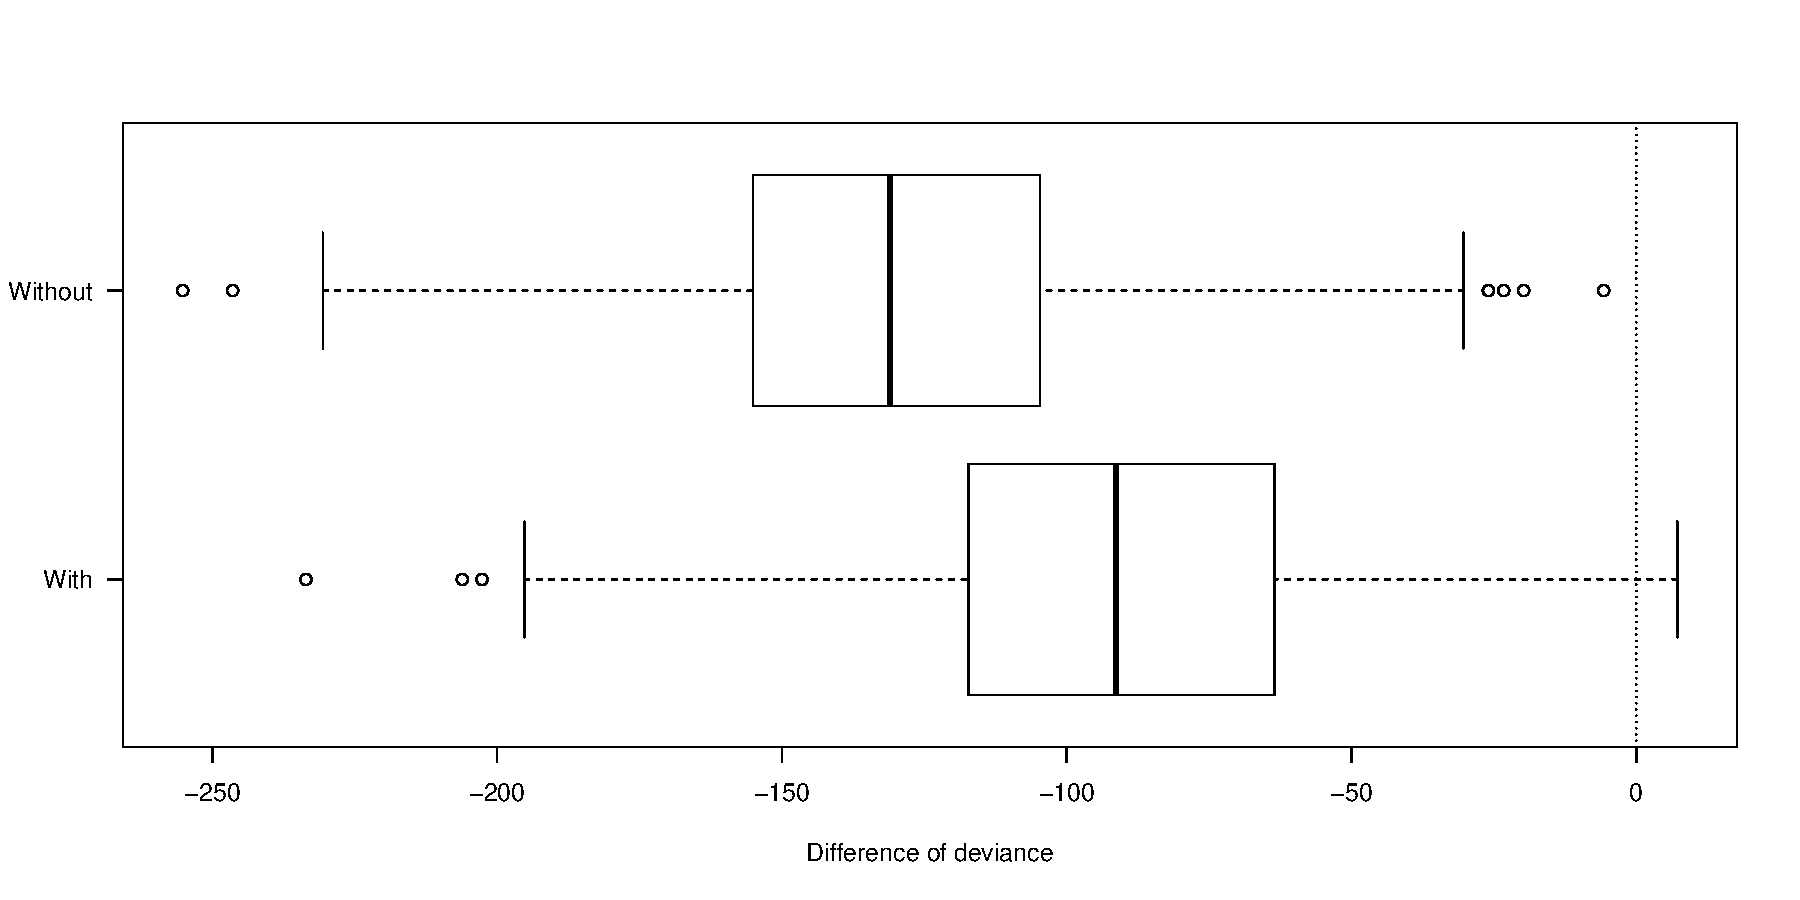
\includegraphics[scale=0.4]{deviances_simulation.pdf}
\end{figure}

\subsubsection{Variable selection}
Let us contrast the two versions of FHTBoost in terms of variable selection as well.
This scenario has 35 informative gene covariates and 5 informative clinical covariates.
Since the changing intercept version has a rather low number of iterations, with a mean of 15.8, it is usually impossible to get anywhere near perfect on these metrics, as at most one new parameter is selected in each iteration, and we have 40 informative covariates in total from the two vectors.
Since the covariate vector is estimated on the training data, a likely explanation is that the changing intercept captures more of the variation in the training data.
In doing so, there is less variation to be explained by the covariates, and hence the boosting algorithm will start to overfit more quickly.

Furthermore, we are considering the sensitivity and specificity on both covariate vectors at the same time.
Since we are only selecting a covariate for either $\bbeta$ or $\bgamma$, these scores will depend on each other.

\begin{table}
\caption{High dimensional (genomic) part: Performance of FHTBoost in terms of variable selection, uncorrelated case}
\label{table:uncorrelated-y0}
\centering
\begin{tabular}{l|cc|cc}
\toprule
& \multicolumn{2}{c}{Updating} & \multicolumn{2}{c}{Fixed} \\
& Mean & Standard error & Mean & Standard error \\
\hline
Sensitivity & 0.190 & (0.090) & 0.452 & (0.162) \\
Specificity & 1.000 & (0.000) & 0.997 & (0.002) \\
FDR         & 0.310 & (0.176) & 0.613 & (0.144) \\
\bottomrule
\end{tabular}
\end{table}

\begin{table}
\caption{Low dimensional (clinical) part: Performance of FHTBoost in terms of variable selection, uncorrelated case}
\label{table:uncorrelated-mu}
\centering
\begin{tabular}{l|cc|cc}
\toprule
& \multicolumn{2}{c}{Updating} & \multicolumn{2}{c}{Fixed} \\
& Mean & Standard error & Mean & Standard error \\
\hline
Sensitivity & 0.741 & (0.232) & 0.958 & (0.099) \\
Specificity & 0.943 & (0.110) & 0.638 & (0.291) \\
FDR         & 0.091 & (0.144) & 0.375 & (0.192) \\
\bottomrule
\end{tabular}
\end{table}

\begin{table}
\caption{Optimal iteration number $\mstop$ results for FHTBoost, uncorrelated case}
\label{table:uncorrelated-mstop}
\centering
\begin{tabular}{l|rr}
\toprule
& Updating & Fixed \\
\hline
Mean               &  15.8  &  63.8  \\
Standard deviation &   6.4  &  26.5  \\
Minimum            &     2  &     2  \\
Maximum            &    39  &   160  \\
\bottomrule
\end{tabular}
\end{table}

Consider first the result of the version in which the intercept is changed in each step.
Both covariate vectors have a very high specificity, which measures the amount of true negatives which are correctly classified as negatives, i.e., not selected.
The changing intercept version has a mean specificity of 1.00.
It also has a mean false discovery rate of 0.316.
Thus there is about a one in three chance that it selects a variable which is not actually informative.
The sensitivity, i.e., the ratio of correctly selected informative variables, has a mean of only 0.190.
This means that a large proportion of the informative covariates are not selected.
For $\bgamma$, which is related to the clinical covariates, a much higher specificity is attained, with a mean of 0.943.
Even though the parameter effects on the drift are rather small, the informative covariates are often correctly selected.
Furthermore, the false discovery rate here is very low, with a mean of 0.091.

Now consider the results of the fixed intercept version.
For the $\bbeta$ covariate vector, a higher proportion of informative covariates are selected, with a mean sensitivity of 0.452.
The mean specificity is 0.997.
Simultaneously, a larger mean false discovery rate of 0.613 is not good:
This means that more than half of all selected variables should be expected to be false positives.
At the same time, a very good sensitivity is achieved on the $\bgamma$ covariate vector, with a mean of 0.958, and a good specificity with a mean of 0.638.
The false discovery rate on $\bgamma$ is slightly above one in three, with a mean of 0.375.

\subsubsection{Summary}
\todo[inline]{Summarize}

\subsection{Scenario 2: Correlated case}
We now consider the results for the correlated simulation study.

\subsubsection{Test set performance/model fit}
We observe that the mean deviance is very slightly better for the fixed intercept version, and with better extreme values, both minimum and maximum.
See Figure \ref{fig:simulation-correlated-deviances-boxplot} for a boxplot of these deviances.
However, it is very close, so it is difficult to say that there is any difference in the model fit for these two versions.

\begin{figure}
\caption{Boxplot for difference in deviance for the two intercept variants, correlated scenario}
\label{fig:simulation-correlated-deviances-boxplot}
\centering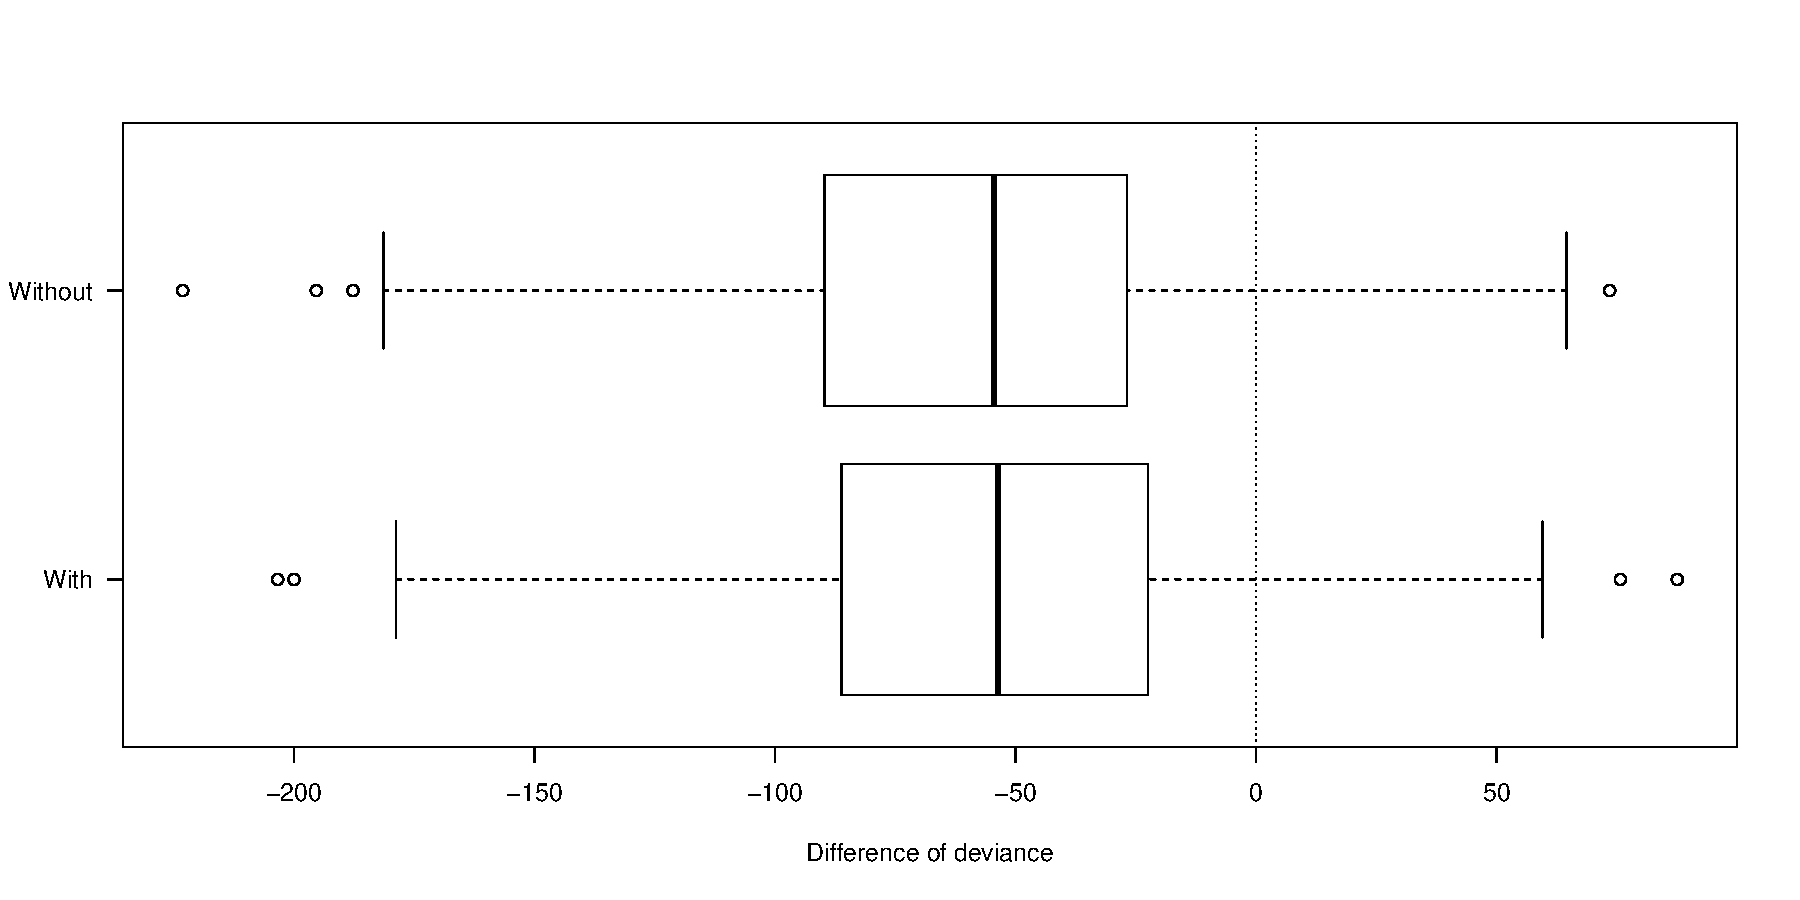
\includegraphics[scale=0.4]{deviances_simulation_correlated.pdf}
\end{figure}


\begin{table}
\caption{Difference of deviance results for FHTBoost, correlated case}
\label{table:uncorrelated-deviance}
\centering
\begin{tabular}{l|rr}
\toprule
& Updating & Fixed \\
\hline
Mean               &  -57.8  &  -58.8  \\
Standard deviation &   47.2  &   46.1  \\
Minimum            & -203.4  & -223.1  \\
Maximum            &   87.6  &   73.5  \\
\bottomrule
\end{tabular}
\end{table}


\subsubsection{Variable selection}
We now consider the variable selection metrics.
We first look at the covariate vector $\bbeta$, which affects the initial level $y_0$, and which is related to ``genomic'' variables.
The fixed intercept version is slightly better with regards to sensitivity, with a mean of 0.204 versus a mean of 0.157 for the changing intercept version.
So selecting informative variables,
This does come at the cost of a higher false discovery rate, with a mean as high as 0.652.
Here the changing intercept version has a mean of 0.439.
The specificity score is almost perfect in both cases.

We now consider the ``clinical'' covariates, used in $\bgamma$ and related to the drift $\mu$.
The changing intercept version performs quite a lot worse here than the fixed intercept version, overall.
It achieves a mean sensitivity of 0.273, while the fixed intercept version achieves 0.625.
However, the changing intercept then achieves a mean of 0.831 for specificity, where the fixed intercept version attains 0.537.
For the false discovery rate, the fixed intercept has a slightly higher mean, at 0.507, whereas the changing intercept version has a mean of 0.454.

For this scenario, as well, we see that the fixed intercept version has a higher optimal iteration number.
The mean $\mstop$ is 50 with a fixed intercept, compared to a mean of 19.5 for the changing intercept version.
Again this necessarily means that more variables are selected, and that coefficients from the changing intercept version will be more shrunken.

\begin{table}
\caption{High dimensional (genomic) part: Performance of FHTBoost in terms of variable selection, correlated case}
\label{table:correlated-y0}
\centering
\begin{tabular}{l|cc|cc}
\toprule
& Updating & & Fixed & \\
& Mean & Standard error & Mean & Standard error \\
\hline
Sensitivity & 0.157 & (0.084) & 0.204 & (0.081) \\
Specificity & 0.999 & (0.000) & 0.998 & (0.001) \\
FDR         & 0.439 & (0.218) & 0.652 & (0.181) \\
\bottomrule
\end{tabular}
\end{table}

\begin{table}
\caption{Low dimensional (clinical) part: Performance of FHTBoost in terms of variable selection, correlated case}
\label{table:correlated-mu}
\centering
\begin{tabular}{l|cc|cc}
\toprule
& Updating & & Fixed & \\
& Mean & Standard error & Mean & Standard error \\
\hline
Sensitivity & 0.273 & (0.187) & 0.625 & (0.245) \\
Specificity & 0.831 & (0.139) & 0.537 & (0.236) \\
FDR         & 0.454 & (0.250) & 0.507 & (0.130) \\
\bottomrule
\end{tabular}
\end{table}

\begin{table}
\caption{Optimal iteration number $\mstop$ results for FHTBoost, correlated case}
\label{table:correlated-mstop}
\centering
\begin{tabular}{l|rr}
\toprule
& Updating & Fixed \\
\hline
Mean               &  20.0  &  51.1  \\
Standard deviation &  12.1  &  24.4  \\
Minimum            &     2  &     2  \\
Maximum            &    65  &   148  \\
\bottomrule
\end{tabular}
\end{table}

\subsubsection{Conclusion}
In conclusion, while the fixed intercept version also here selects more true positive variables, it comes at a cost of selecting more false positives.
If we use the deviance to assess which one is best, then the fixed intercept version is the better one here as well.

\section{Discussion}
In general, we see that FHTBoost is able to estimate FHT models which achieve good performance, on data generated from a true FHT mechanism.
The performance achieved is especially high for the uncorrelated scenario.
As we have discussed, the variable selection has trade offs.
The fixed intercept version selects more true positives, but it also selects more false positives.
It does seem to be worth it, in the end, since it achieves a better generalization error in the form of a lower difference of deviance.
The results are also good in the highly correlated scenario.
Since this is a much more realistic scenario, we should give more weight to the results attained in it.
If so, it is difficult to make a conclusive statement on which version is better, as the results are very similar in the highly correlated scenario.
However, to narrow down the scope of the analysis in the next chapter, we will decide to only use the fixed intercept version, as we at least cannot say that it is not better than the changing intercept version.